\documentclass[iop]{emulateapj}
\usepackage{epstopdf}
\usepackage{epsfig}
\usepackage{natbib}
%\usepackage{lscape}
%\usepackage{deluxetable}
%\usepackage{rotating}

\citestyle{aa} 
\bibliographystyle{apj}
\def\Nstars{1040}
\def\msun{\mbox{$M_\odot$}}
\def\lsun{\mbox{$L_\odot$}}
\def\rsun{\mbox{$R_\odot$}}
\def\tsun{\mbox{$T_\odot$}}
\def\teff{\mbox{$T_{\rm eff}$}}
\def\logg{\mbox{$\log g$}}
\def\fe{\mbox{[Fe/H]} }
\def\Mbolsun{\mbox{$M_{\rm bol,\odot}$}}
\def\Loggsun{\mbox{$\log g_\odot$}}
\def\LogLsun{\mbox{$\log L_\odot$}}
\def\etal{\mbox{\rm et al.~}}
\def\cms{\mbox{cm s$^{-1}$}}
\def\ms{\mbox{m s$^{-1}$}}
\def\kms{\mbox{km s$^{-1}$}}
\def\msy{\mbox{m s$^{-1}$ yr$^{-1}$}}
\def\ks{\mbox{km s$^{-1}$}}
\def\cse{\mbox{cm s$^{-2}$}}
\def\mstar{M$_{\star}$}
\def\rstar{R$_{\star}$}
\def\mjup{$M_{\rm Jup}$}
\def\mearth{$M_{\oplus}$}
\def\msat{M$_{\rm SAT}$}
\def\rjup{$R_{\rm Jup}$}
\def\vsini{$v \sin i$}
\def\msini{$M_{P} \sin{i}$}
\def\mbsini{$M_b \sin{i}$}
\def\mcsini{$M_c \sin{i}$}
\def\chisq{$\sqrt{\chi_{\nu}^2}$}
\def\arel{$a_{\rm rel}$}
\def\hipp{$Hipparcos$ }
\def\snr{\mbox{\rm signal-to-noise}}
\def\caii{\ion{Ca}{2}}
\def\shk{\mbox{$S_{\rm HK}$}}
\def\chinu{$\chi_{\nu}^{2}$~}
\def\plm{$\pm$\ }
\def\sme{$\mathcal{SME}$}

\def\rms{RMS}
\def\snrfit{SNR}


%VARIABLES
\def\cbers{\texttt{CHI\_BISECTORS~}}
\def\cbis{\texttt{CHI\_BISECT~}}
\def\acenb{$\alpha$ Centauri B}

%MJG Commands:
\def\tc{$t_{c}$}

\textwidth 6.5in
%\voffset=0.3in  % This is because the printer I use prints too low...
\def\baselinestretch{0.96}

%\received{?}
%\accepted{2013}

\shorttitle{CHIRON Efficiency}
\shortauthors{Giguere et al.}
\begin{document}

\title{CHIRON Efficiency as of August 2013}

\author{Matthew J. Giguere\altaffilmark{1}}	

\begin{abstract}
This document discusses the efficiency of CHIRON after the GAM mirror cleaning and tip-tilt module installation. The efficiency was calculated by observing 3 secondary standards on the night of 130801. We find that the efficiency was largely unchanged relative to the efficiency calculation from June 2012. The median efficiency between 5000 and 6000 \AA was 6.5 \%.

\end{abstract}

\keywords{instrumentation}

\altaffiltext{1}{Department of Astronomy, Yale University, 260 Whitney Ave, New Haven, CT 06511, USA}
\ \


\section{Introduction}
In April of 2013 a new tip-tilt module was installed in the front end module (FEM) of CHIRON with the goal of improving guiding on Alpha Cen A \& B. While the tip-tilt was being installed, it was discovered that the mirror on the guider-acquisition module (GAM) had a thick layer of dust on it. Both the cleaning of the GAM mirror and the installation of the tip-tilt module were expected to have increased the throughput of CHIRON. This work discusses a new calculation of the efficiency of CHIRON.

\section{Observations \& Reduction}

To determine the efficiency of CHIRON, 3 secondary standards were observed that were selected from \citep{1992PASP..104..533H, 1994PASP..106..566H} based on the seasonal observability of the targets in August. All observations were taken on August 1st, 2013. The Yale Bright Star Catalog (HR) numbers of the chosen targets, along with spectral types, B and V apparent magnitudes, and mean airmass when observed are listed in Table \ref{tab:targets}. All exposures were taken in the unmasked fiber mode to maximize throughput. The data were extracted using the standard CHIRON reduction pipeline that all CHIRON observations are processed through, which extracts from 4500 \AA~to 8800 \AA.

%% The values (usually only l,r and c) in the last part of
%% \begin{deluxetable}{} command tell LaTeX how many columns
%% there are and how to align them.
\begin{deluxetable}{ccccc}

%% Keep a portrait orientation

%% Over-ride the default font size
%% Use Default (12pt)

%% Use \tablewidth{?pt} to over-ride the default table width.
%% If you are unhappy with the default look at the end of the
%% *.log file to see what the default was set at before adjusting
%% this value.

%% This is the title of the table.
\tablecaption{Secondary Standards Observed for Efficiency Calculation \label{tab:targets}}

%% This command over-rides LaTeX's natural table count
%% and replaces it with this number.  LaTeX will increment 
%% all other tables after this table based on this number
\tablenum{1}

%% The \tablehead gives provides the column headers.  It
%% is currently set up so that the column labels are on the
%% top line and the units surrounded by ()s are in the 
%% bottom line.  You may add more header information by writing
%% another line between these lines. For each column that requries
%% extra information be sure to include a \colhead{text} command
%% and remember to end any extra lines with \\ and include the 
%% correct number of &s.
\tablehead{\colhead{OBJECT} & \colhead{Sp} & \colhead{B} & \colhead{V} & \colhead{Airmass}} 

%% All data must appear between the \startdata and \enddata commands
\startdata
HR 7596 &  A0III & 5.704 &  5.628 &  1.563 \\
HR 8634 &  B8V & 3.313 &  3.390 &  1.328 \\
HR 9087 &  B7III-IV & 4.998 &  5.119 &  1.353 \\
\enddata

%% Include any \tablenotetext{key}{text}, \tablerefs{ref list},
%% or \tablecomments{text} between the \enddata and 
%% \end{deluxetable} commands

%% No \tablecomments indicated

%% No \tablerefs indicated

\end{deluxetable}

\section{Methods}

The standard CHIRON reduction pipeline applies the gain to convert counts to photoelectrons. The final product of each reduced observation is a FITS file with 2 layers: the first layer being the wavelength solution based on the nearest ThAr exposure taken in the respective mode, and the second layer being the spectrum, in photoelectrons. To convert from photoelectrons to monochromatic flux, $f_{\nu}$, in erg~cm$^{-2}$~s$^{-1}$~Hz$^{-1}$, the following equation was used

\begin{equation}
f_{\nu} = \frac{n_{\gamma} h c}{A w \lambda t_{exp} }
\end{equation}

where $n_{\gamma}$ is the number of photoelectrons per pixel, h is Planck's constant, $\lambda$ is the wavelength corresponding to each pixel, A is the area of the telescope, w is the width of each pixel in frequency space, and $t_{exp}$ is the exposure time. The total light gathering area of the 1.5 m is 13135 cm$^{2}$, which takes into account the secondary obstruction, which is 0.38 m in radius.

\citet{1994PASP..106..566H} list the monochromatic magnitudes in 16 \AA~ steps from 3300\AA~ to 10420 \AA~ for each of these 3 stars. To convert from monochromatic magnitudes to monochromatic fluxes, the same zero point was used as in their work.

\begin{equation}
f_{\nu} = 10^{-0.4(m_{\nu} + 48.590)}
\end{equation}

For each of the 62 orders, the blaze peak was determined using the max value of the polynomial fit to each order in the master flat. The monochromatic flux at blaze peak was then determined by taking the median value of the seven pixels nearest to the blaze peak. The atmospheric extinction correction was calculated by performing a cubic spline interpolation to the wavelength corresponding to blaze peak from the extinction curve for CTIO from \citep{Stritzinger:2005dt}, which is shown in Figure \ref{fig:extinction}.

\begin{figure}[ht]
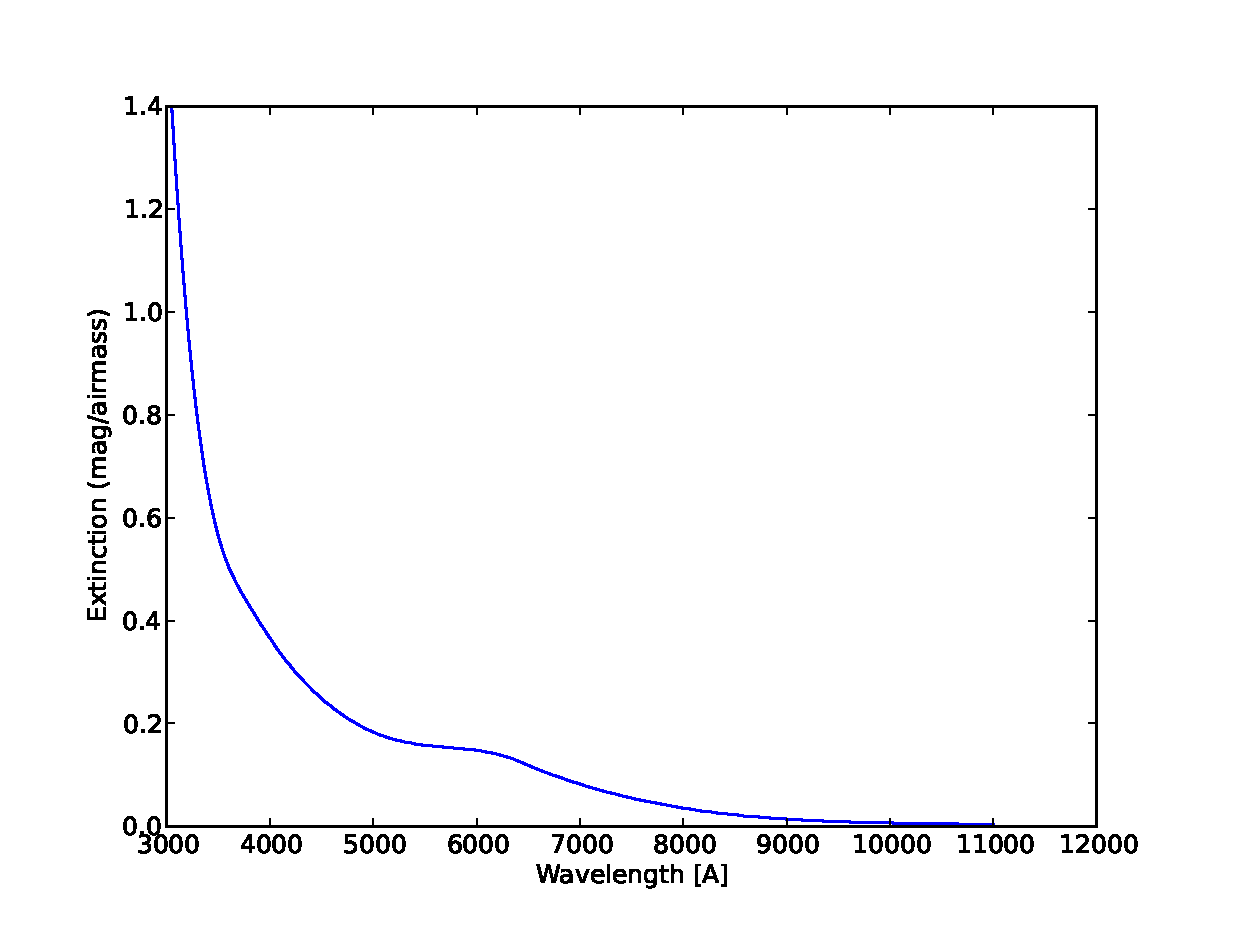
\includegraphics[scale=0.4,angle=0]{fig_Exinction.eps}
\caption{\label{fig:extinction} The atmospheric extinction from \citet{Stritzinger:2005dt}, as seen from CTIO.}
\end{figure}

The monochromatic flux with the atmospheric extinction taken into account, $f_{cor}$, is then

\begin{equation}
f_{cor} = f_{\nu}10^{0.4m_{ext}}
\end{equation}

The efficiency was then calculated by taking a ratio of $f_{cor}$ to the monochromatic flux from \citep{1994PASP..106..566H}, where again a cubic spline interpolation was used to get the monochromatic flux at the wavelength corresponding to blaze peak. The results for HR~7596, HR~8634, and HR~9087 can be seen in Figures \ref{fig:hr7596}, \ref{fig:hr8634}, and \ref{fig:hr9087}, respectively. 

\section{Results \& Discussion}

After calculating the efficiency as a function of wavelength for all the wavelengths at blaze peak, a median overall efficiency was computed by taking of the median efficiency value of the 9 results at each wavelength element. The result can be seen, plotted over all nine curves in Figure \ref{fig:effall}, and alone in Figure \ref{fig:medeff}. This shows a median efficiency between 5000 \AA~and 6000 \AA~of 6.5\%, with a peak of 6.6\% at 5600\AA. Comparing this result to the efficiency calculation from June 13, 2012, the overall efficiency of CHIRON after cleaning the GAM mirror and inclusion of a tip-tilt mechanism has not changed significantly. 

While the telescope operator reported conditions as clear, with 1"-1".2 seeing, there was large variability between observations. There was a comment in the end of night report from the night these observations were taken stating there were problems with dome movement. This large variability could have been due to occultation of the dome, or perhaps overpassing cirrus during the efficiency observations. It would be useful to take additional observations of at least one of the targets on a separate clear night without dome movement failures to confirm the calculated efficiency.  

\begin{figure}[ht]
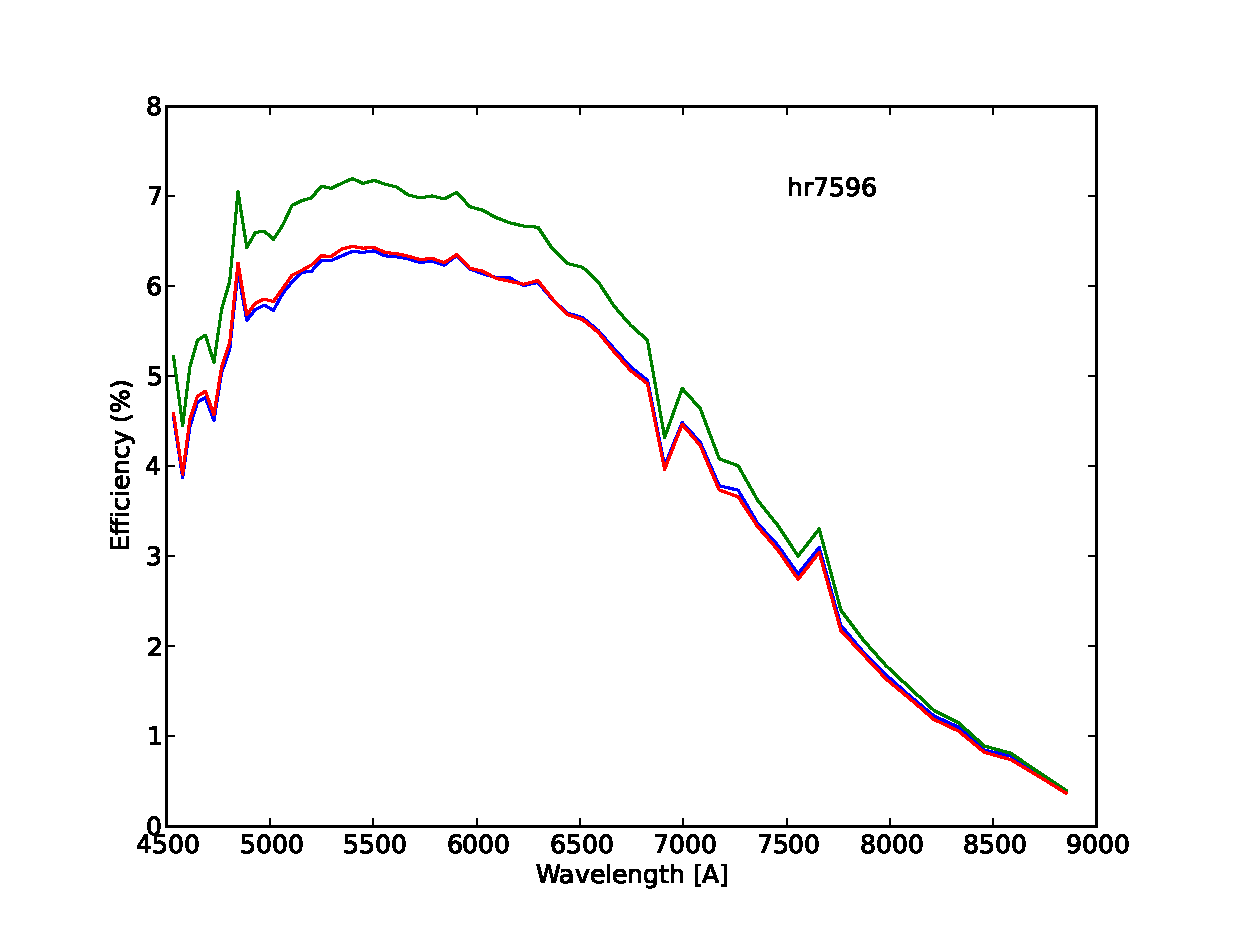
\includegraphics[scale=0.4,angle=0]{fig_eff_hr7596_all.eps}
\caption{\label{fig:hr7596} The efficiency of CHIRON based on 3 observations of HR~7596, a bright secondary standard star, all taken on August 1st, 2013.}
\end{figure}

\begin{figure}[ht]
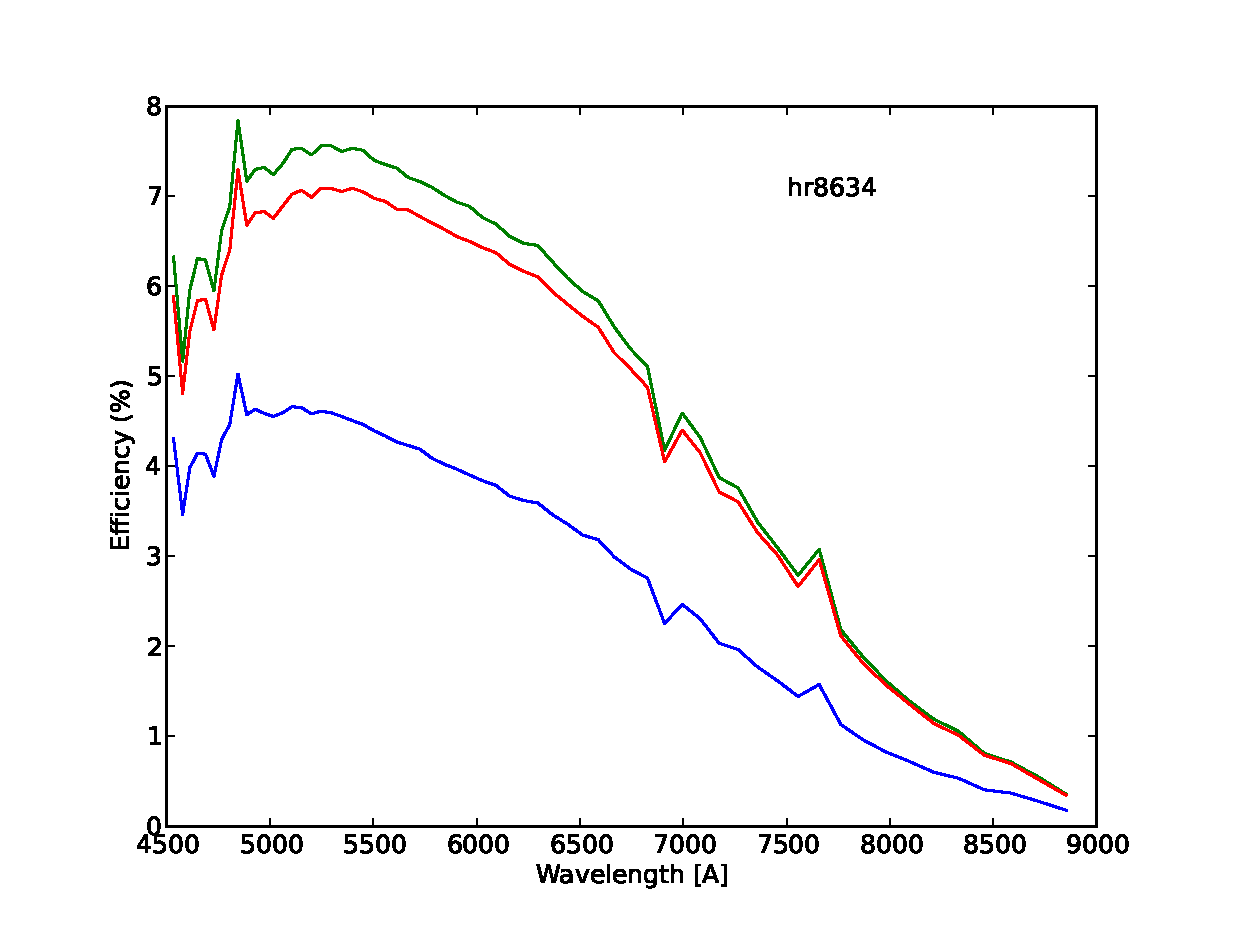
\includegraphics[scale=0.4,angle=0]{fig_eff_hr8634_all.eps}
\caption{\label{fig:hr8634} The efficiency of CHIRON based on 3 observations of HR~8634, a bright secondary standard star, all taken on August 1st, 2013.}
\end{figure}

\begin{figure}[ht]
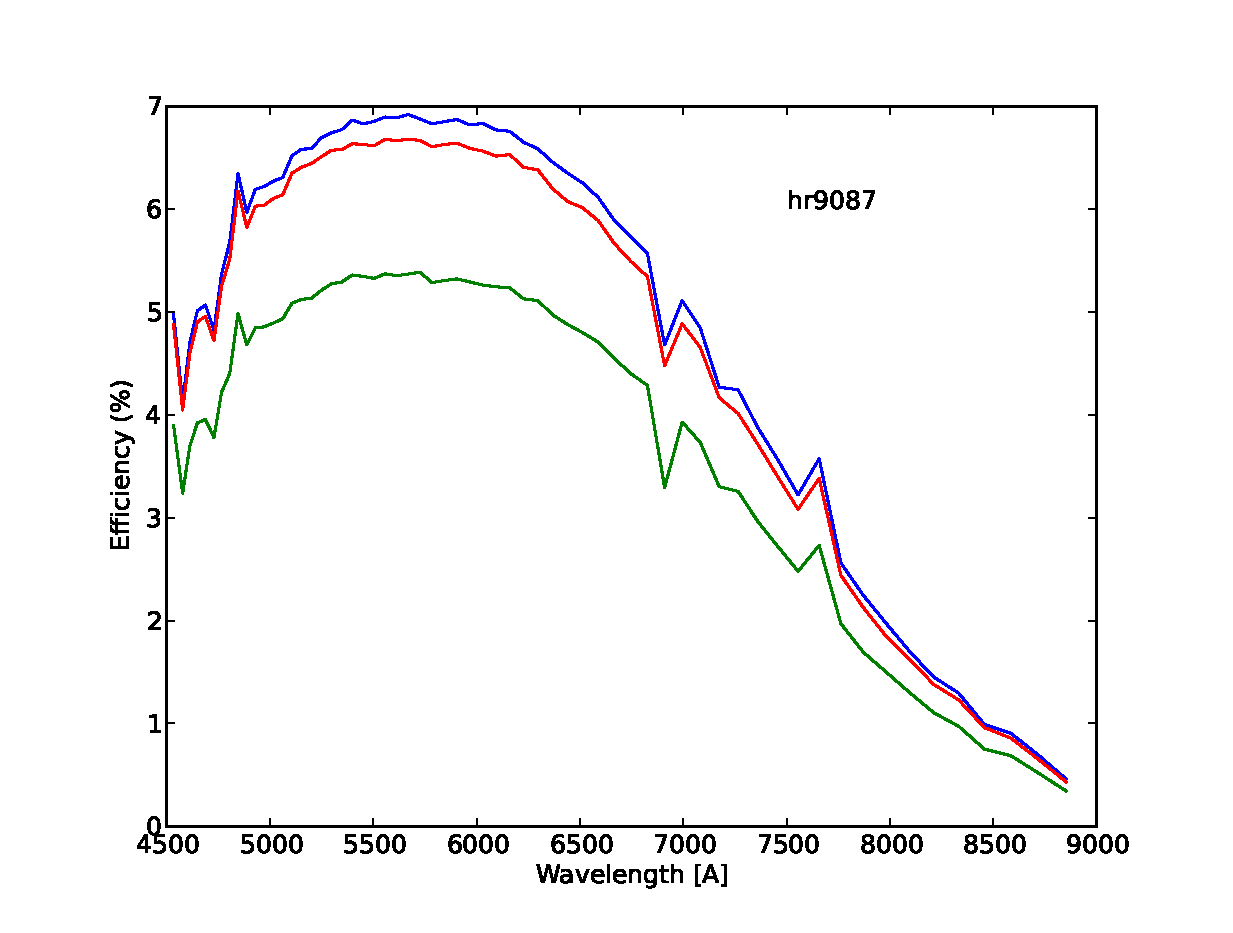
\includegraphics[scale=0.4,angle=0]{fig_eff_hr9087_all.eps}
\caption{\label{fig:hr9087} The efficiency of CHIRON based on 3 observations of HR~9087, a bright secondary standard star, all taken on August 1st, 2013.}
\end{figure}

\begin{figure}[ht]
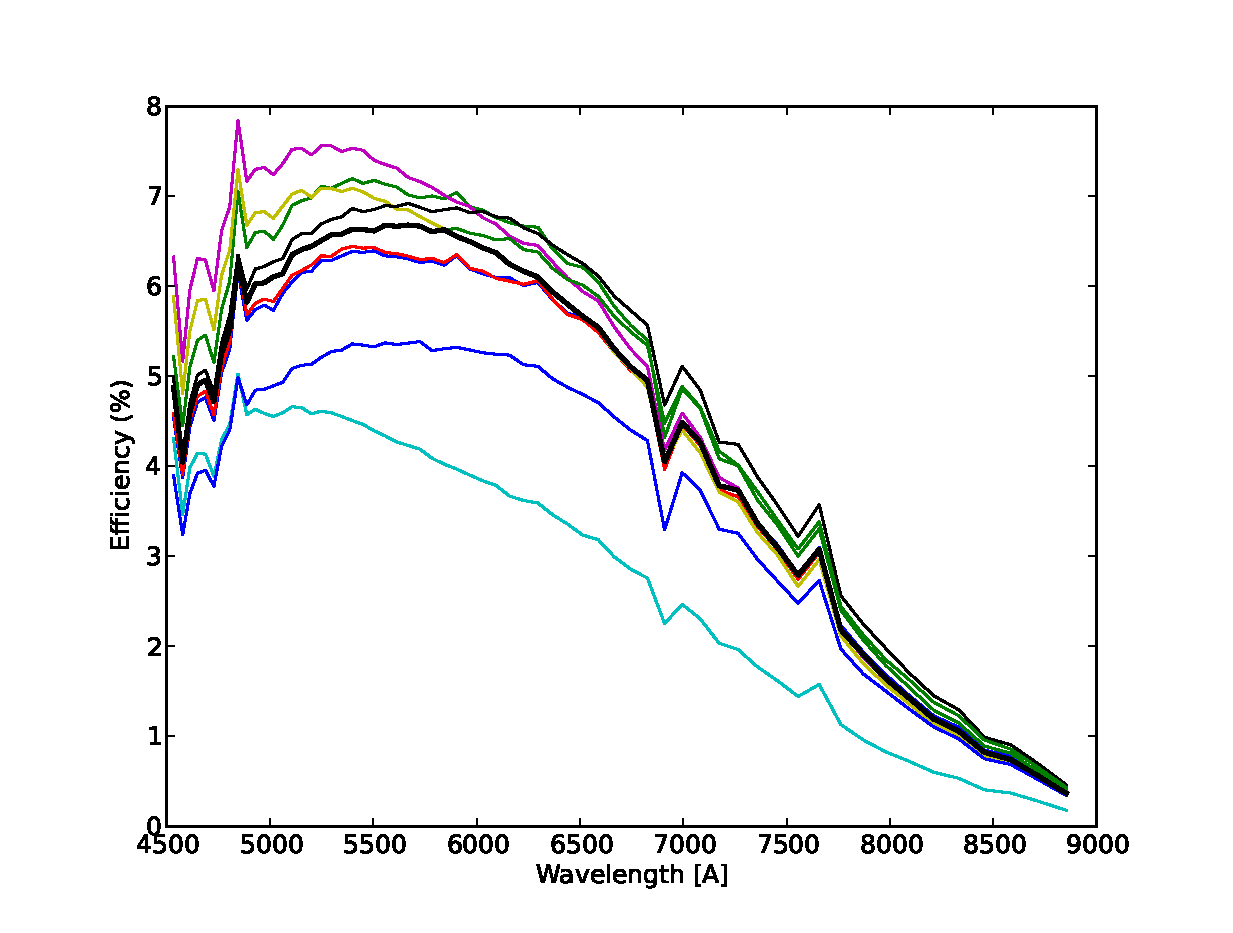
\includegraphics[scale=0.4,angle=0]{fig_medeff_all.eps}
\caption{\label{fig:effall} The combined CHIRON efficiency calculation of all 9 exposures (3 of each of the 3 targets). The thick black line is the median of all 9 exposures.}
\end{figure}

\begin{figure}[ht]
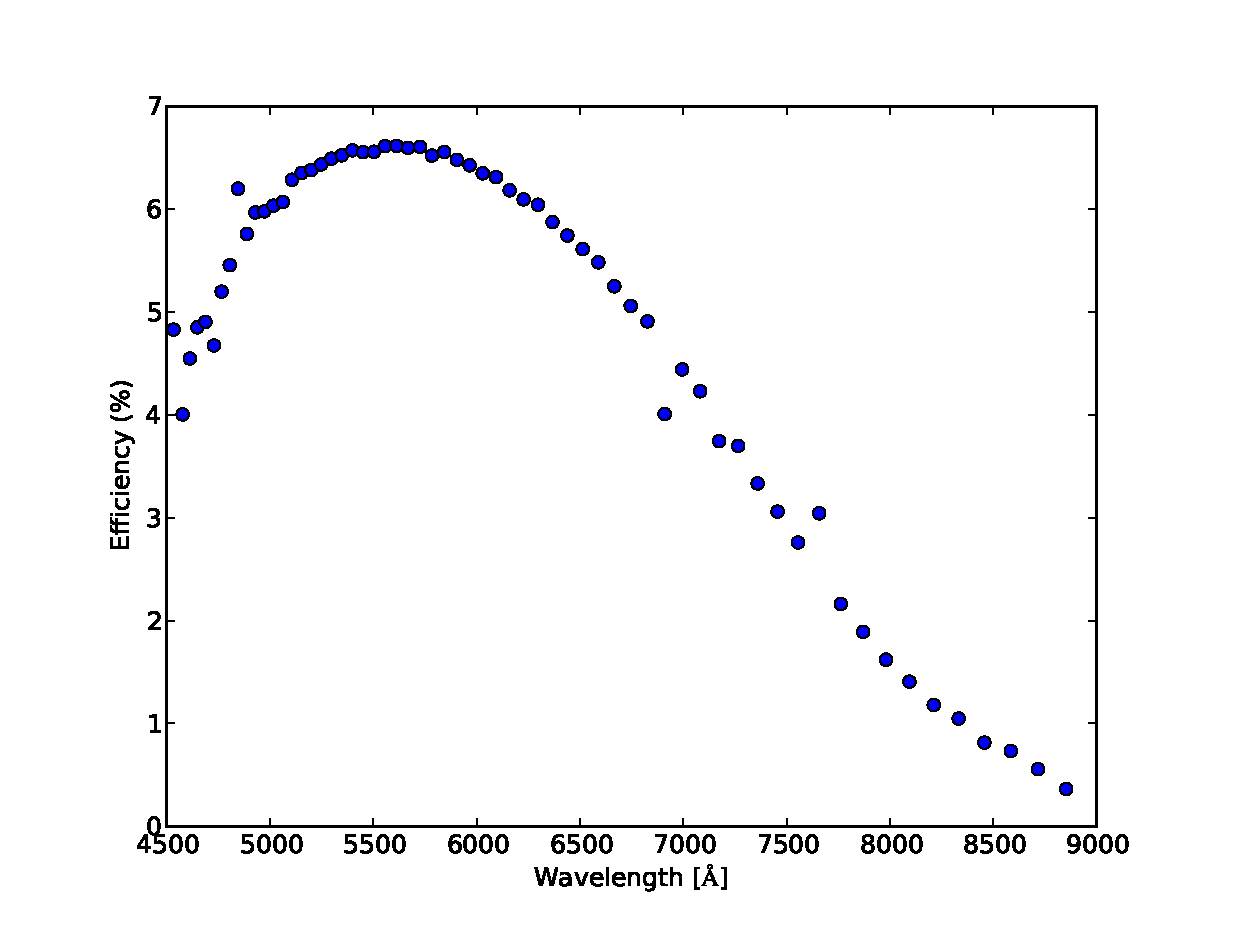
\includegraphics[scale=0.4,angle=0]{fig_medeff.eps}
\caption{\label{fig:medeff} The combined median CHIRON efficiency based on 9 exposures (3 exposures each of 3 targets). The median efficiency between 5000 and 6000 \AA~was 6.5\%.}
\end{figure}


\section{Acknowledgements}
This research has made use of the SIMBAD database,
operated at CDS, Strasbourg, France.

\bibliographystyle{apj}
\bibliography{apj-jour,biblib_chirps}

%%%%%%%%%%%%%%%%%%%%%%%%%%%%%%%%%%%%%%%%%%%%%%%%
%%%                                                                 TABLES                                                                         %%%
%%%%%%%%%%%%%%%%%%%%%%%%%%%%%%%%%%%%%%%%%%%%%%%%

%%%%%%%%%%%%%%%%%%%%%%%%%%%%%%%%%%%%%%%%%%%%%%%%
%%%                                                                 FIGURES                                                                       %%%
%%%%%%%%%%%%%%%%%%%%%%%%%%%%%%%%%%%%%%%%%%%%%%%%

\clearpage

\clearpage
\end{document}
